\documentclass[main.tex]{subfiles}
\begin{document}
\section{Dataset}
The dataset consists of time series data showing power consumption over 32 different European countries\footnote{https://data.open-power-system-data.org/time\_series/} shown in megawatts in hourly steps starting from the 1st of January 2015 and ending on the 30th of September 2020. This amounts to 50400 hours of time series data, which is roughly 5.7 years. \\
Below the whole dataset is shown, and a clear seasonality is seen in the data, with the most power consumption being around the winter seasons.
\begin{figure}[H]
\centering
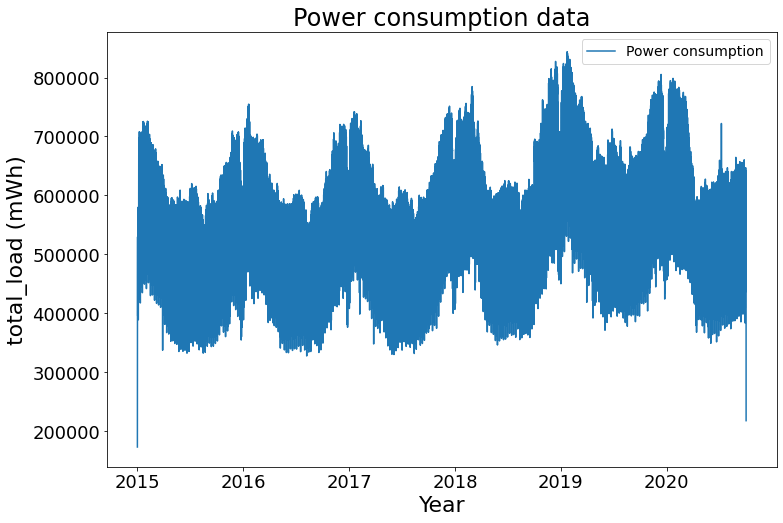
\includegraphics[width=0.6\textwidth]{GeneralPlots/powerdata.png}
\label{fig:fulldataplot}
\caption{Plot of the whole dataset}
\end{figure}
For the purpose of evaluating different methods for time series forecasting, the most important use of this dataset did not lie in differentiating between power consumption from the different European countries or delve into the waters of multi-variate predictions. But rather to use the dataset as a whole as a stepping stone, and simplify the problem, so that the focus could be on evaluating the different models, and more easily compare them to each other. For this the specific features showing power consumption from the different countries were extracted and summed them up to have one feature, \textit{total load}, thus turning the problem into a single feature problem as apposed to multi-variate prediction.\\
\\
Furthermore, the data was subsampled, which means that the hourly data was turned into daily data. This serves the purpose of keeping the data at a decent size, not removing to many data points, while still being able to see some interesting dynamics from timestep to timestep. As shown below, the power consumption can be seen fluctuating on a weekly basis, while still keeping in line with the seasonality and overall trend of the whole dataset. 

\begin{figure}[H]
\centering
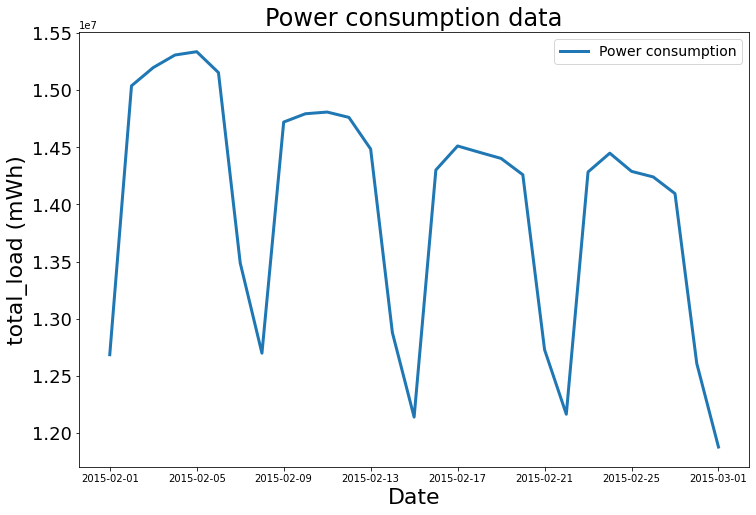
\includegraphics[width=0.6\textwidth]{GeneralPlots/powerdata2.png}
\label{fig:daily_plot}
\caption{Approximately a month's worth of daily data}
\end{figure}

Throughout the project, the dataset is augmented into what is called a time series dataset. This method is general across different models, and is what makes it possible to train both the simple and advanced model, and to make not only single-step predictions but also multi-step prediction.\\
The method consists of making data sequences of sources and targets, which are sequences of time series data taken from the dataset, where the target sequence is shifted a number of steps, corresponding to the wanted prediction length.\\
In the case of the simple model, the source can be viewed as the training input and target is the wanted output which is what the actual output of the model is compared to. In the case of the advanced model, as it is an encoder-decoder architecture, the model needs both source and target for training.
\begin{figure}[H]
    \centering
    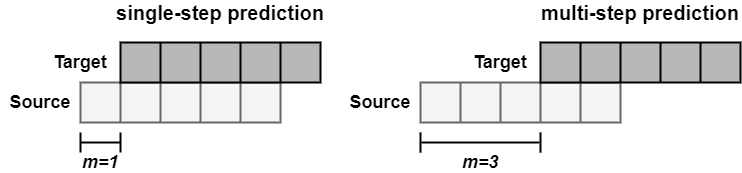
\includegraphics[width=0.9\textwidth]{Figures/timeseriesfigure.png}
    \caption{Visualization of data sequences for single-step and multi-step prediction}
    \label{fig:timeseriesfigure}
\end{figure}

\end{document}